\documentclass{../../slides-style}

\slidetitle{Лекция 2: О жизненном цикле и методологиях}{27.02.2024}

\begin{document}

    \begin{frame}[plain]
        \titlepage
    \end{frame}

    \section{Жизненный цикл}

    \begin{frame}
        \frametitle{Виды деятельности при разработке ПО}
        \begin{itemize}
            \item Возникновение и исследование идеи
            \item Анализ и сбор требований (пилотный проект)
            \item Планирование и проектирование
            \item Разработка
            \item Отладка и тестирование
            \item Сдача
            \item Сопровождение
        \end{itemize}
    \end{frame}

    \begin{frame}
        \frametitle{Жизненный цикл ПО}
        \begin{itemize}
            \item Период времени от возникновения идеи до прекращения использования
            \item Последовательность этапов
            \begin{itemize}
                \item Состав и последовательность работ
                \item Получаемые результаты
                \item Методы и средства
                \item Роли и ответственности
                \item \dots
            \end{itemize}
            \item Модели жизненного цикла
        \end{itemize}
    \end{frame}

    \section{Модели ЖЦ}

    \begin{frame}
        \frametitle{Самая популярная модель разработки ПО}
        \begin{center}
            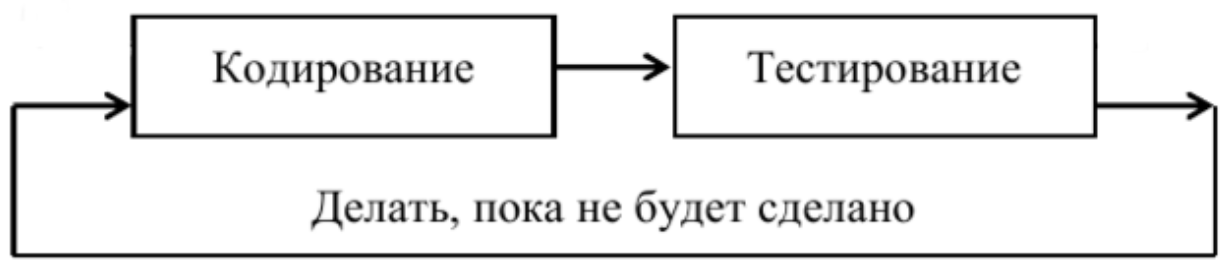
\includegraphics[width=0.6\textwidth]{cowboyCodingModel.png}
        \end{center}
    \end{frame}

    \begin{frame}
        \frametitle{Водопадная (каскадная) модель}
        \begin{center}
            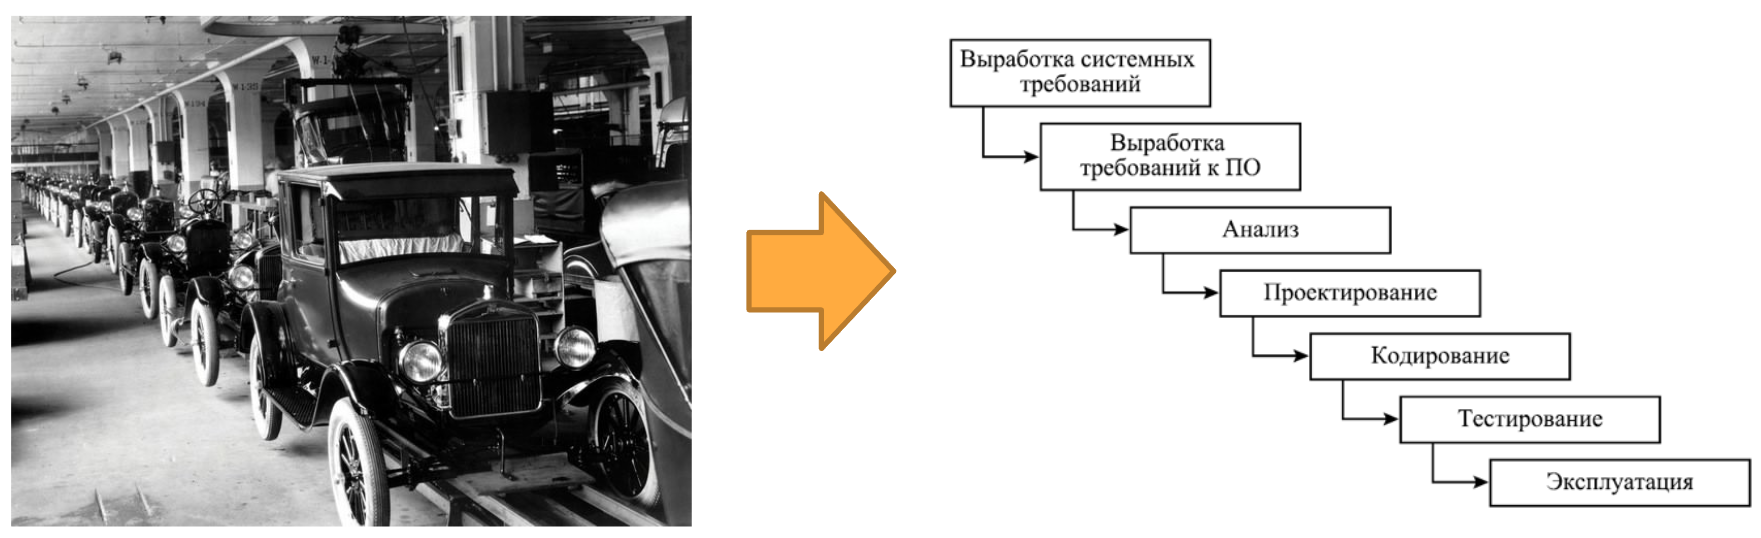
\includegraphics[width=\textwidth]{waterfallAndConveyor.png}
        \end{center}
        В. Ройс, 1970г, ``Managing the Development of Large Software Systems''
    \end{frame}

    \begin{frame}
        \frametitle{Водопадная (каскадная) модель}
        \begin{center}
            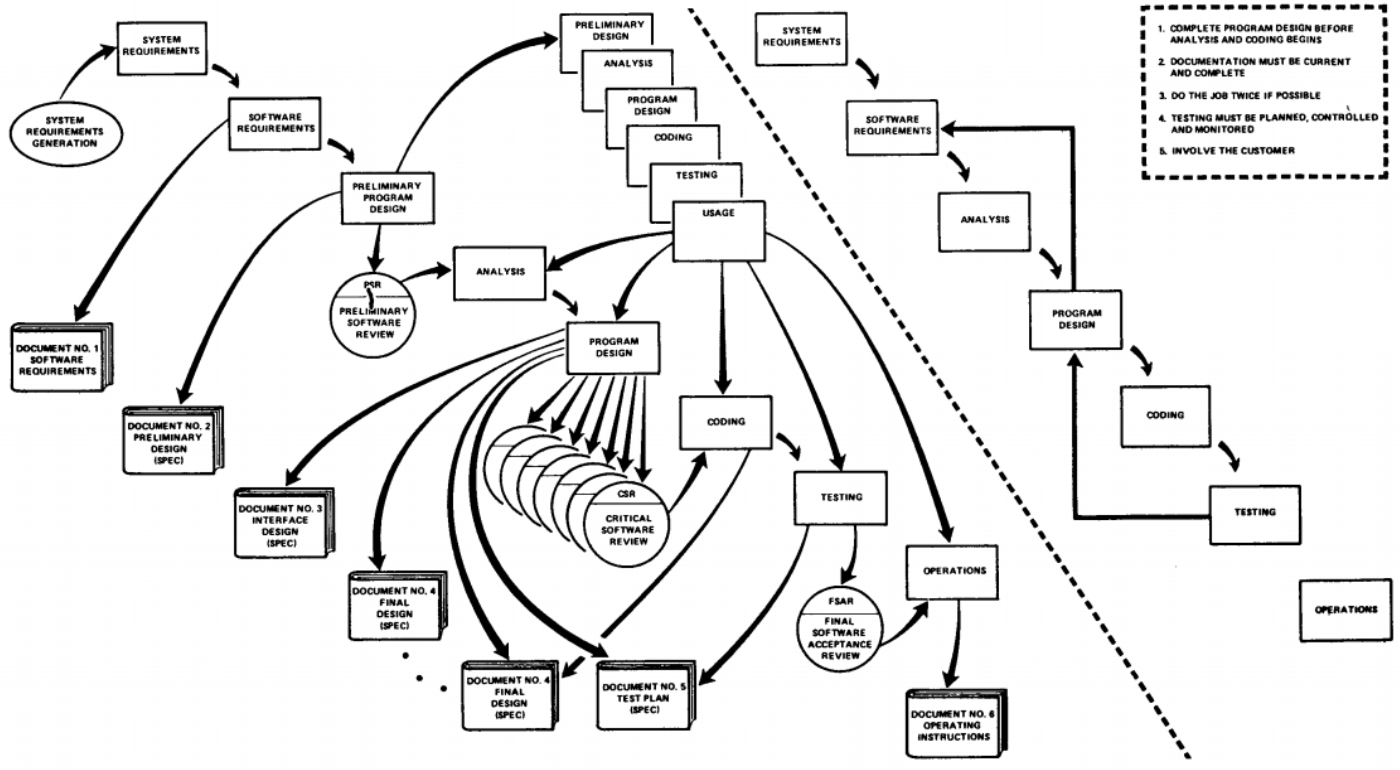
\includegraphics[width=\textwidth]{waterfallDetailed.png}
        \end{center}
    \end{frame}

    \begin{frame}
        \frametitle{Водопадная (каскадная) модель}
        \begin{center}
            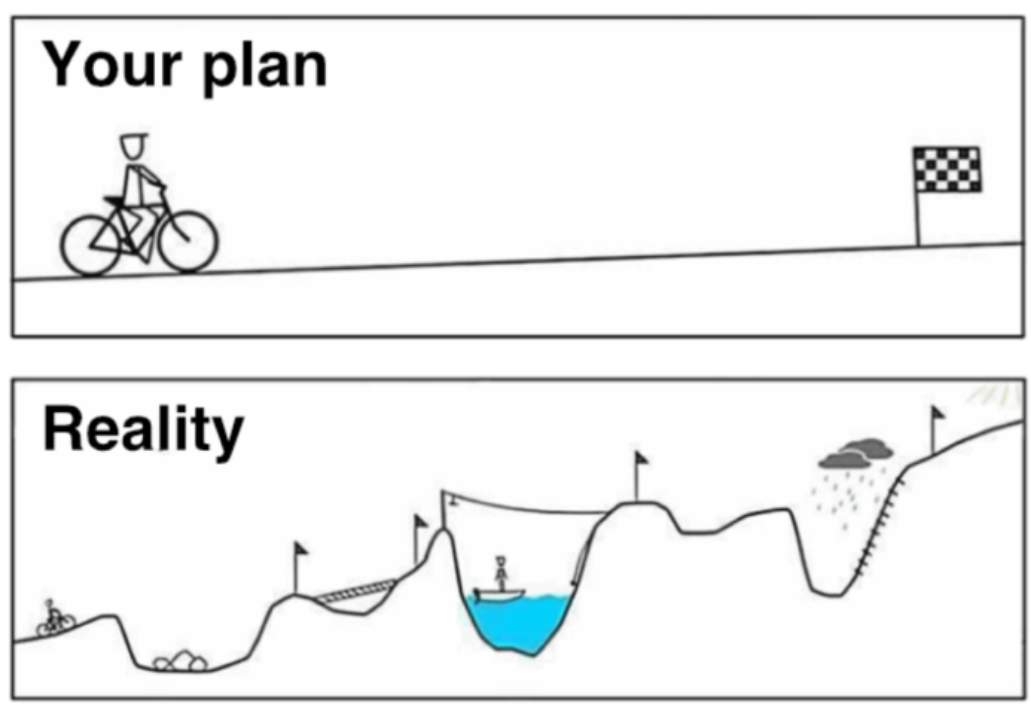
\includegraphics[width=0.6\textwidth]{waterfallProblems.png}
        \end{center}
    \end{frame}

    \begin{frame}
        \frametitle{Итеративная модель}
        \begin{center}
            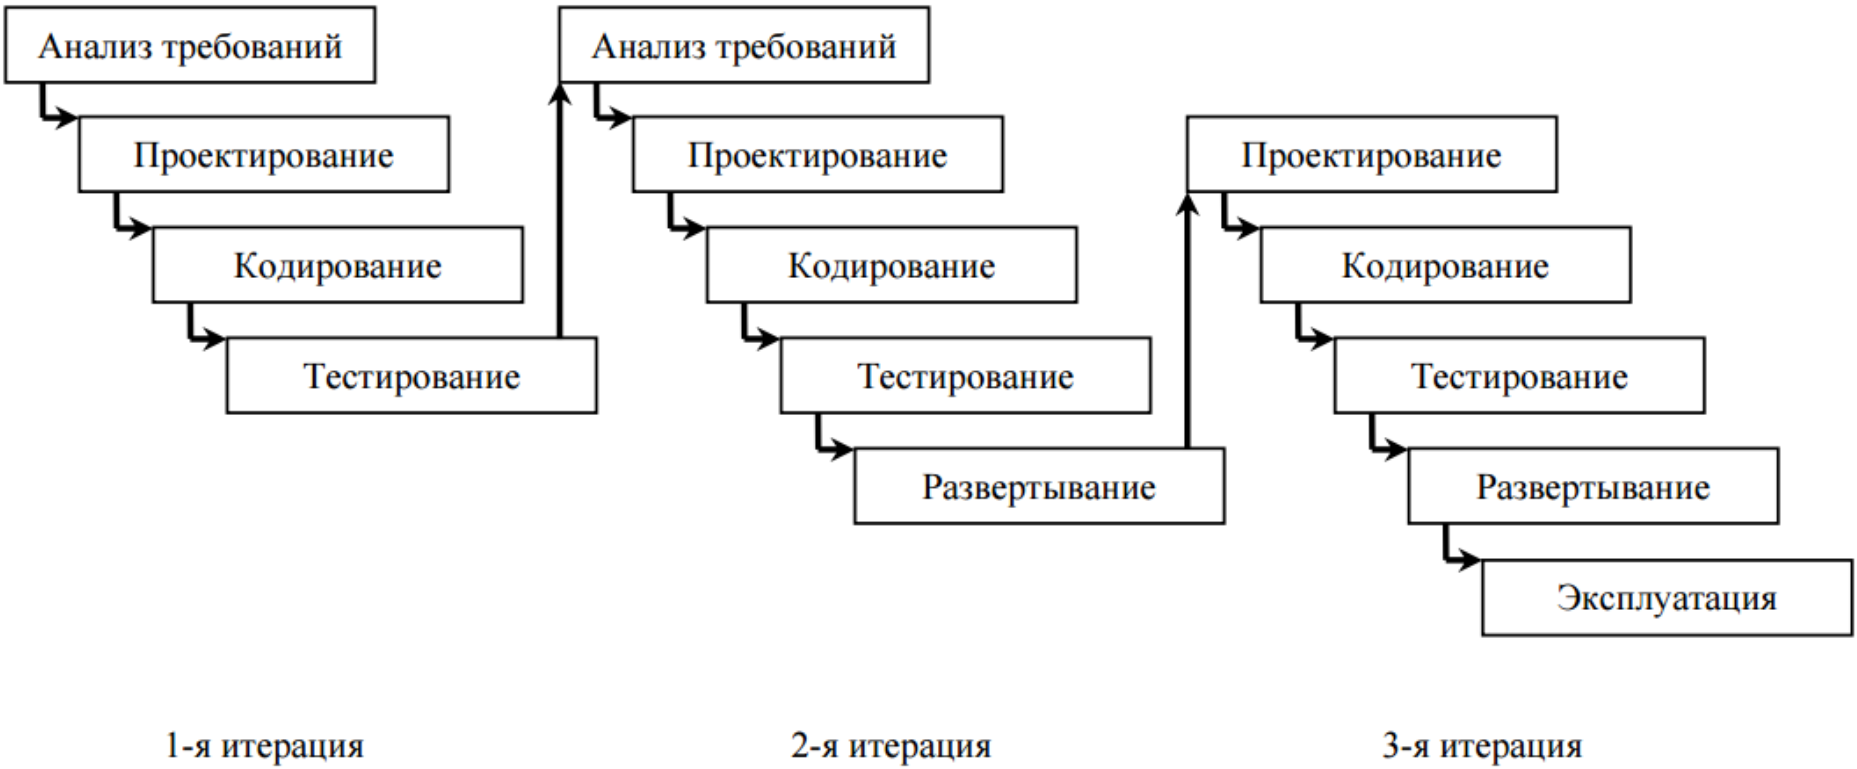
\includegraphics[width=0.9\textwidth]{iterativeModel.png}
        \end{center}
    \end{frame}

    \begin{frame}
        \frametitle{Итеративно-инкрементальная модель}
        \begin{center}
            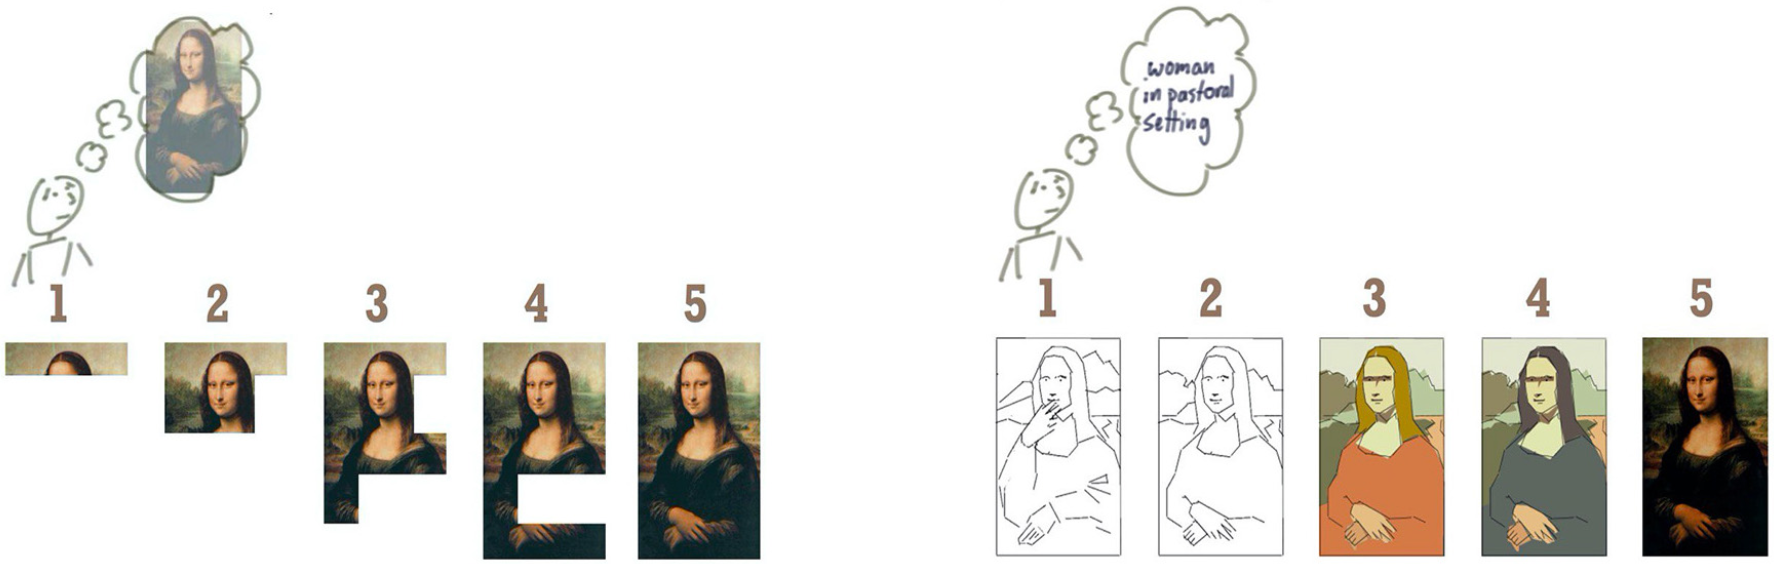
\includegraphics[width=0.9\textwidth]{iterativeIncrementalModel.png}
        \end{center}
    \end{frame}

    \begin{frame}
        \frametitle{Спиралевидная модель}
        \begin{center}
            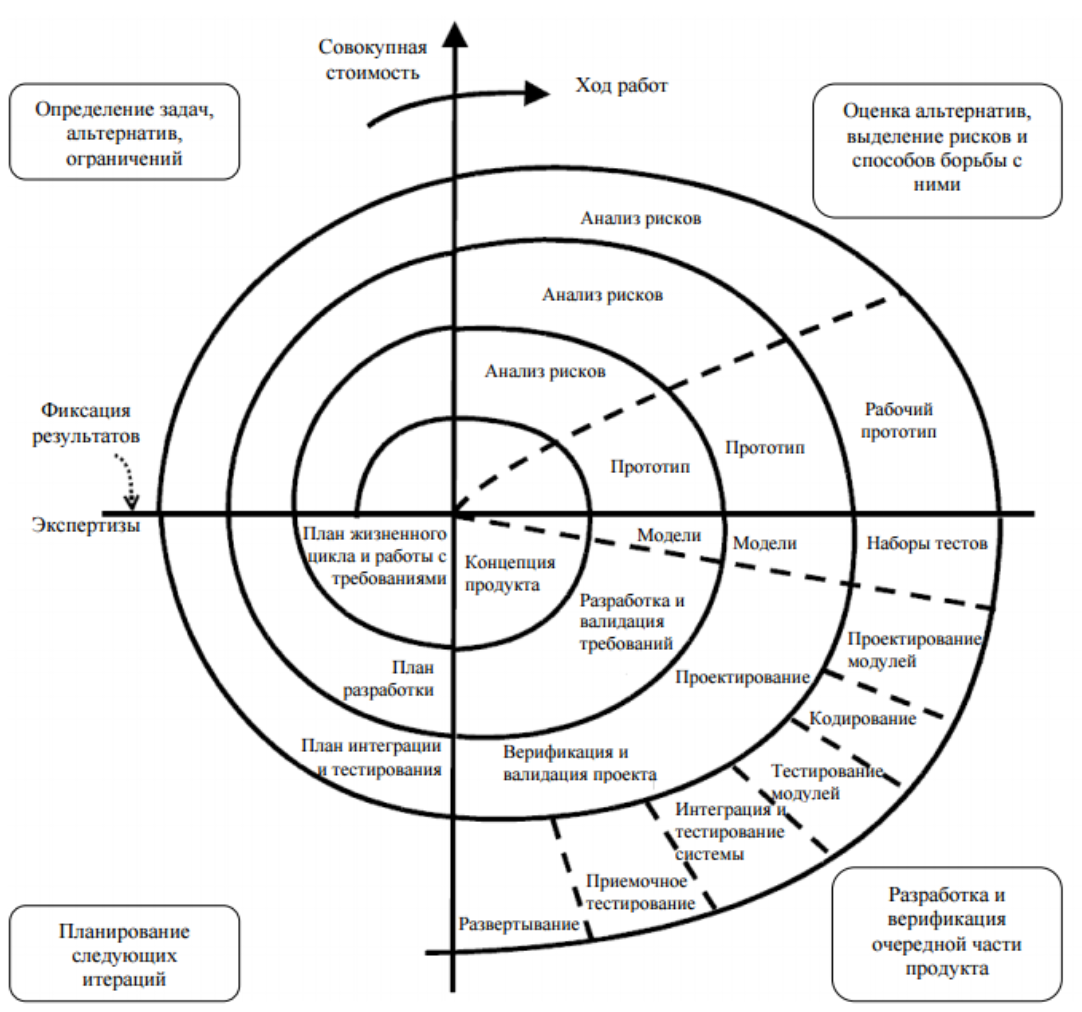
\includegraphics[width=0.6\textwidth]{spiralModel.png}
        \end{center}
    \end{frame}

    \begin{frame}
        \frametitle{The Lean Startup Model}
        \begin{center}
            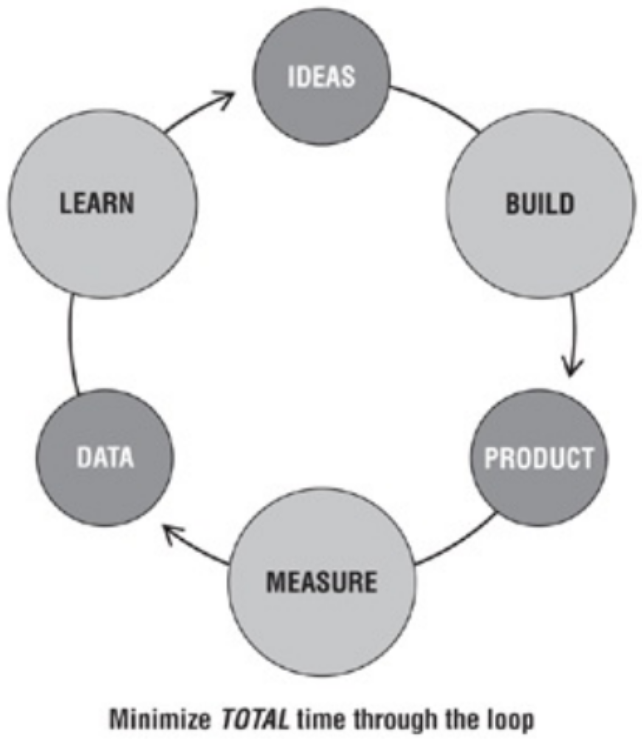
\includegraphics[width=0.4\textwidth]{theLeanStartupModel.png}
        \end{center}
    \end{frame}

    \section{RUP}

    \begin{frame}
        \frametitle{Rational Unified Process (RUP)}
        \begin{columns}
            \begin{column}{0.5\textwidth}
                \begin{itemize}
                    \item Пример ``тяжёлого'' процесса разработки
                    \begin{itemize}
                        \item Отделение практик от людей
                    \end{itemize}
                    \item Ivar Jacobson, 1980-е годы
                    \item Ericsson/Objectory AB/Rational
                    \item Основные идеи:
                    \begin{itemize}
                        \item варианты использования
                        \item архитектура, архитектура, архитектура
                        \item управляемые итерации
                    \end{itemize}
                \end{itemize}
            \end{column}
            \begin{column}{0.5\textwidth}
                \begin{center}
                    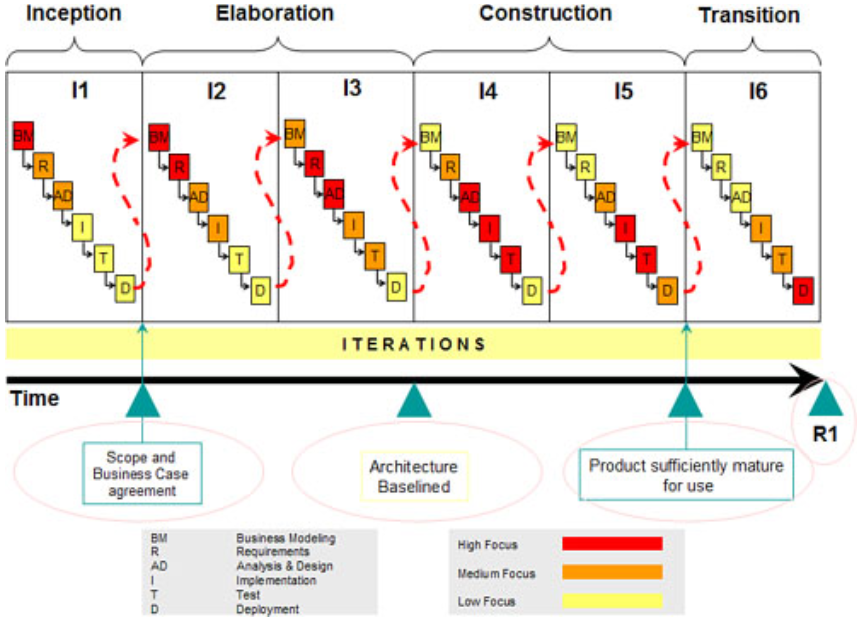
\includegraphics[width=\textwidth]{rup.png}
                \end{center}
            \end{column}
        \end{columns}
    \end{frame}

    \begin{frame}
        \begin{center}
            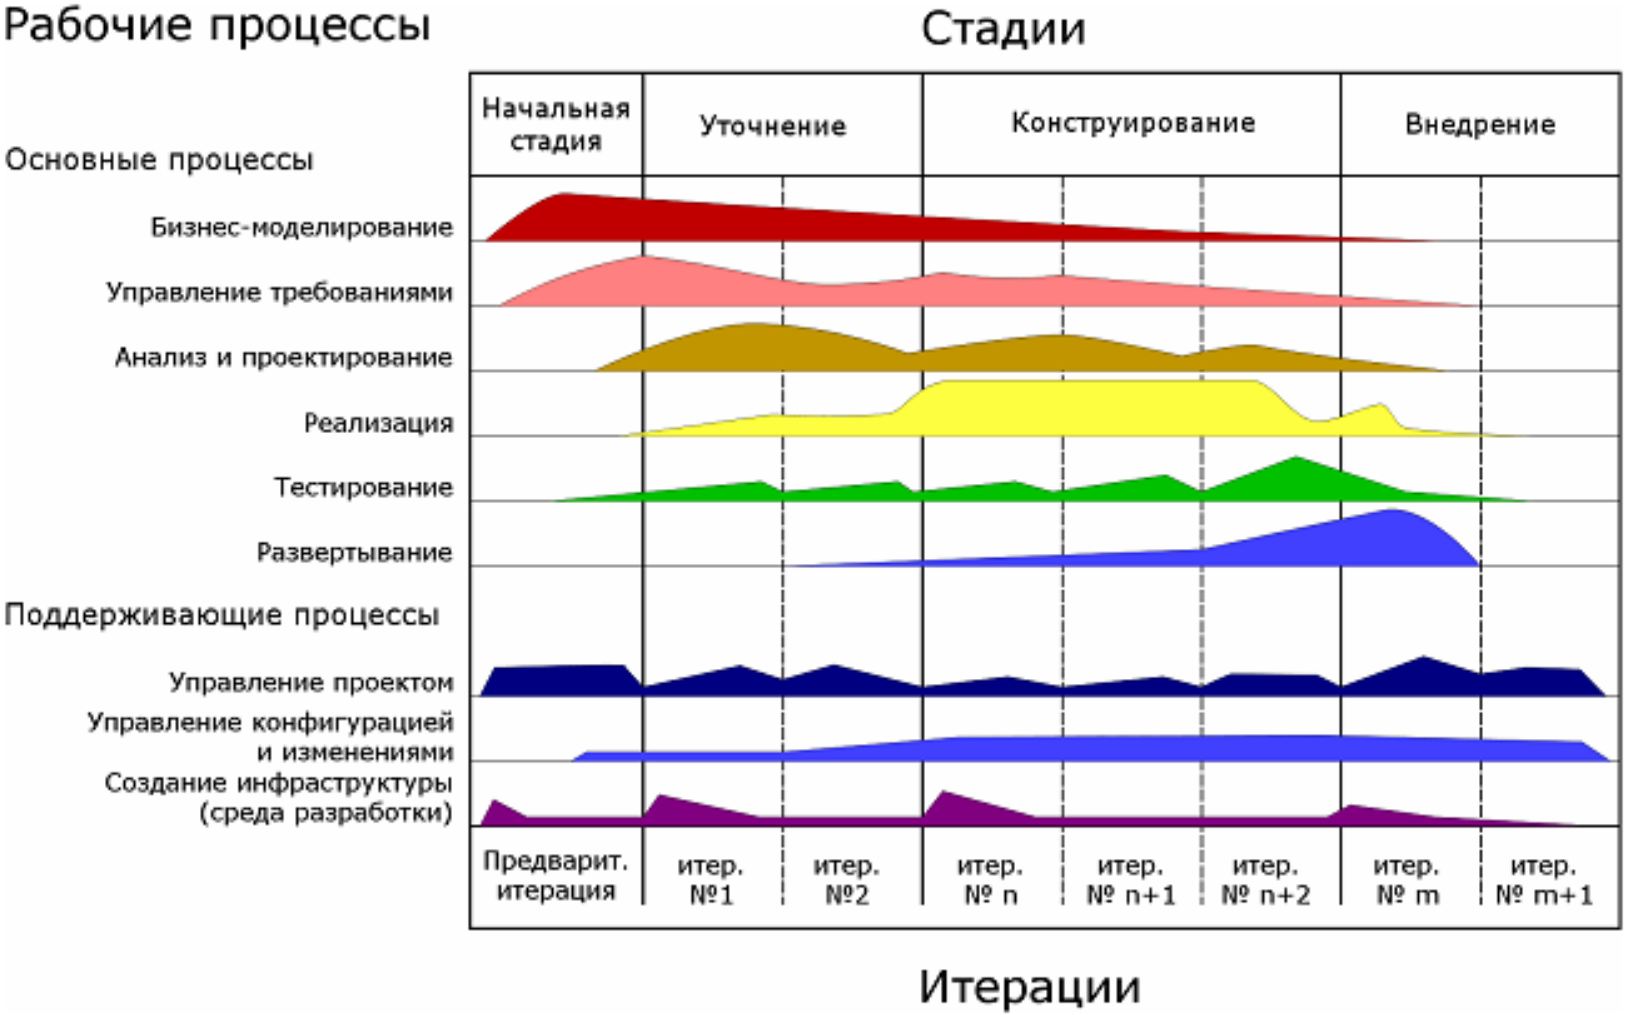
\includegraphics[width=0.9\textwidth]{rupProcesses.png}
        \end{center}
    \end{frame}

    \begin{frame}
        \frametitle{Модели, создаваемые в RUP}
        \begin{itemize}
            \item Модель случаев использования
            \item Модель анализа (концептуальная модель)
            \item Модель проектирования
            \item Модель реализации
            \item Модель развёртывания
            \item Модель тестирования
        \end{itemize}
    \end{frame}

    \begin{frame}
        \frametitle{Принципы RUP}
        \begin{itemize}
            \item Выработка концепции проекта (project vision) в его начале
            \item Управление по плану
            \item Снижение рисков и отслеживание их последствий
            \item Тщательное экономическое обоснование всех действий
            \item Как можно более раннее формирование базовой архитектуры
            \item Использование компонентной архитектуры
            \item Прототипирование, инкрементная разработка и тестирование
            \item Регулярные оценки текущего состояния
            \item Управление изменениями
            \item Нацеленность на создание работоспособного продукта
            \item Нацеленность на качество
            \item Адаптация процесса под нужды проекта
        \end{itemize}
    \end{frame}

    \section{Agile}

    \begin{frame}
        \begin{center}
            
\includegraphics[width=\textwidth]{agileManifesto.png}
        \end{center}
        \begin{small}
            \url{http://agilemanifesto.org/iso/ru/manifesto.html}
        \end{small}
    \end{frame}

    \begin{frame}
        \frametitle{12 принципов Agile (1)}
        \begin{enumerate}
            \item Удовлетворение клиента за счёт ранней и бесперебойной поставки ценного программного обеспечения
            \item Приветствие изменений требований даже в конце разработки (это может повысить конкурентоспособность полученного продукта)
            \item Частая поставка рабочего программного обеспечения (каждый месяц или неделю или ещё чаще)
            \item Тесное, ежедневное общение заказчика с разработчиками на протяжении всего проекта
        \end{enumerate}
    \end{frame}

    \begin{frame}
        \frametitle{12 принципов Agile (2)}
        \begin{enumerate}
            \setcounter{enumi}{4}
            \item Проектом занимаются мотивированные личности, которые обеспечены нужными условиями работы, поддержкой и доверием
            \item Рекомендуемый метод передачи информации~--- личный разговор (лицом к лицу)
            \item Работающее программное обеспечение~--- лучший измеритель прогресса
            \item Инвесторы, разработчики и пользователи должны иметь возможность поддерживать постоянный темп на неопределённый срок
        \end{enumerate}
    \end{frame}

    \begin{frame}
        \frametitle{12 принципов Agile (3)}
        \begin{enumerate}
            \setcounter{enumi}{8}
            \item Постоянное внимание улучшению технического мастерства и удобному дизайну
            \item Простота — искусство не делать лишней работы
            \item Лучшие технические требования, дизайн и архитектура получаются у самоорганизованной команды
            \item Постоянная адаптация к изменяющимся обстоятельствам. Команда должна систематически анализировать возможные способы улучшения эффективности и соответственно корректировать стиль своей работы
        \end{enumerate}
    \end{frame}

    \section{XP}

    \begin{frame}
        \frametitle{eXtreme Programming (XP)}
        \begin{itemize}
            \item Кент Бек, примерно 1999
            \item Первая широкоизвестная agile-методология
            \item Основные принципы: коммуникация, простота, обратная связь, храбрость
            \item Непопулярна сейчас
            \begin{itemize}
                \item Слишком революционные практики
            \end{itemize}
        \end{itemize}
    \end{frame}

    \begin{frame}
        \frametitle{Практики XP}
        \begin{enumerate}
            \item Короткий цикл обратной связи:
            \begin{itemize}
                \item Разработка через тестирование 
                \item Игра в планирование
                \item Заказчик всегда рядом
                \item Парное программирование
            \end{itemize}
        \end{enumerate}
    \end{frame}

    \begin{frame}
        \frametitle{1. Разработка через тестирование}
        \begin{columns}
            \begin{column}{0.7\textwidth}
                \begin{itemize}
                    \item Большое число автоматических тестов
                    \begin{itemize}
                        \item Модульные тесты
                        \item Функциональные тесты
                    \end{itemize}
                    \item 100\% тестов должно проходить всегда
                    \item Тесты как документирование кода
                    \item Тесты как основа для рефакторинга
                    \item Написание тестов перед написанием кода
                \end{itemize}
            \end{column}
            \begin{column}{0.3\textwidth}
                \begin{center}
                    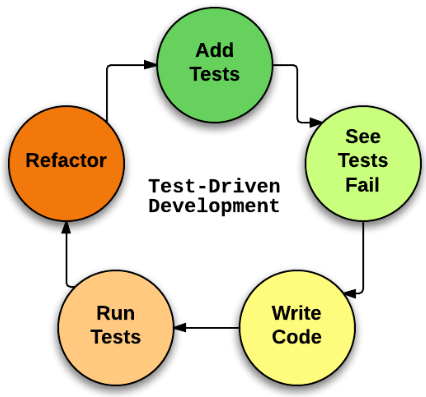
\includegraphics[width=\textwidth]{tddLoop.png}
                \end{center}
            \end{column}
        \end{columns}
    \end{frame}

    \begin{frame}
        \frametitle{2. Игра в планирование}
        \begin{itemize}
            \item Быстро получить приблизительный план работы
            \begin{itemize}
                \item Последовательное уточнение
            \end{itemize}
            \item Идеальное время и load factor
            \item Распределение ответственности между командой и заказчиком
            \begin{itemize}
                \item Приоритизация задач
            \end{itemize}
            \item Customer stories
            \begin{itemize}
                \item Estimatable
                \item Testable
                \item Bite-sizes
                \item Progress
            \end{itemize}
        \end{itemize}
    \end{frame}

    \begin{frame}
        \frametitle{3. Заказчик всегда рядом}
        \begin{itemize}
            \item Представитель пользователей в команде
            \begin{itemize}
                \item Принимает на себя ответственность
                \item Влияет на ход разработки
            \end{itemize}
            \item Снижение затрат на коммуникацию
        \end{itemize}
    \end{frame}

    \begin{frame}
        \frametitle{4. Парное программирование}
        \begin{itemize}
            \item Один компьютер, два программиста
            \begin{itemize}
                \item Регулярное перемешивание пар
            \end{itemize}
            \item Более хороший дизайн и код
            \item Повышение дисциплины
            \item Коллективное владение кодом
            \item Командный дух
            \item Наставничество и обучение
            \item Непрерывная социализация
        \end{itemize}
    \end{frame}

    \begin{frame}
        \frametitle{Практики XP (2)}
        \begin{enumerate}
            \setcounter{enumi}{1}
            \item Непрерывный процесс:
            \begin{itemize}
                \item Непрерывная интеграция 
                \item Рефакторинг 
                \item Частые небольшие релизы
            \end{itemize}
        \end{enumerate}
    \end{frame}

    \begin{frame}
        \frametitle{5. Непрерывная интеграция}
        \begin{itemize}
            \item Частые слияния веток разработки и сборки проекта
            \begin{itemize}
                \item Несколько раз в день
                \begin{itemize}
                    \item По внешнему запросу
                    \item По расписанию
                    \item По событию
                \end{itemize}
            \end{itemize}
            \item Использование систем версионирования кода
            \item Максимальная автоматизация
            \item Постоянное наличие рабочей версии
            \item Затраты на интеграцию
        \end{itemize}
    \end{frame}

    \begin{frame}
        \frametitle{6. Рефакторинг}
        \begin{itemize}
            \item Код постоянно меняется, и это хорошо и правильно
            \item Рефакторинг~--- средство поддержки эволюции
            \begin{itemize}
                \item Долги проектирования
            \end{itemize}
            \item Реализуем только то, что нужно сейчас
            \begin{itemize}
                \item Решаем проблемы по мере поступления
            \end{itemize}
            \item Нужно много хороших тестов
        \end{itemize}
        \begin{center}
            
\includegraphics[width=0.7\textwidth]{hatsRefactoring.png}
        \end{center}
    \end{frame}

    \begin{frame}
        \frametitle{7. Частые небольшие релизы}
        \begin{itemize}
            \item Меньше функциональности
            \begin{itemize}
                \item Проще разрабатывать и тестировать
            \end{itemize}
            \item Быстрее доставка фич заказчику
            \item Быстрее обратная связь от заказчика
            \item Отказ от сдвига релизов
            \begin{itemize}
                \item Урезаем функциональность
            \end{itemize}
        \end{itemize}
    \end{frame}

    \begin{frame}
        \frametitle{Практики XP (3)}
        \begin{enumerate}
            \setcounter{enumi}{2}
            \item Понимание, разделяемое всеми:
            \begin{itemize}
                \item Простота архитектуры
                \item Метафора системы
                \item Коллективное владение кодом
                \item Стандарт кодирования
            \end{itemize}
        \end{enumerate}
    \end{frame}

    \begin{frame}
        \frametitle{8. Простота архитектуры}
        \begin{itemize}
            \item Аллергия на BDUF\footnote{Big Design Up-Front}
            \item Непрерывное проектирование
            \item Самые простые решения
            \begin{itemize}
                \item Ориентация на текущие задачи
                \begin{itemize}
                    \item Простой не значит плохой
                    \item Когда нельзя ничего выкинуть, чтобы не потерять функциональность
                \end{itemize}
                \item Непрерывный рефакторинг в зависимости от условий
            \end{itemize}
            \item Отказ от долгосрочного планирования
        \end{itemize}
    \end{frame}

    \begin{frame}
        \frametitle{9. Метафора системы}
        \begin{itemize}
            \item Единое описание того, как работает система
            \begin{itemize}
                \item Текстовое описание, понятное всем
            \end{itemize}
            \item Замена общепринятой архитектуры
        \end{itemize}
    \end{frame}

    \begin{frame}
        \frametitle{10. Коллективное владение кодом}
        \begin{itemize}
            \item Разделение ответственности за весь код
            \begin{itemize}
                \item Автор кода~--- вся команда
            \end{itemize}
            \item Каждый может менять любой код
            \begin{itemize}
                \item Высокий bus factor 
                \item Высокие требования к команде
            \end{itemize}
        \end{itemize}
    \end{frame}

    \begin{frame}
        \frametitle{11. Стандарт кодирования}
        \begin{itemize}
            \item Единый стандарт написания кода
            \begin{itemize}
                \item Не тратим время на споры о несущественном
            \end{itemize}
            \item Простота изменений, интеграции, рефакторинга
            \item Автоматизация проверок стиля
        \end{itemize}
    \end{frame}

    \begin{frame}
        \frametitle{12. 40-часовая рабочая неделя}
        \begin{itemize}
            \item Авралы и переработки вредны на перспективе
            \begin{itemize}
                \item Работоспособность падает
                \item Выгорание
            \end{itemize}
            \item Жертвенность на работе~--- признак непрофессионализма
        \end{itemize}
    \end{frame}

    \begin{frame}
        \begin{center}
            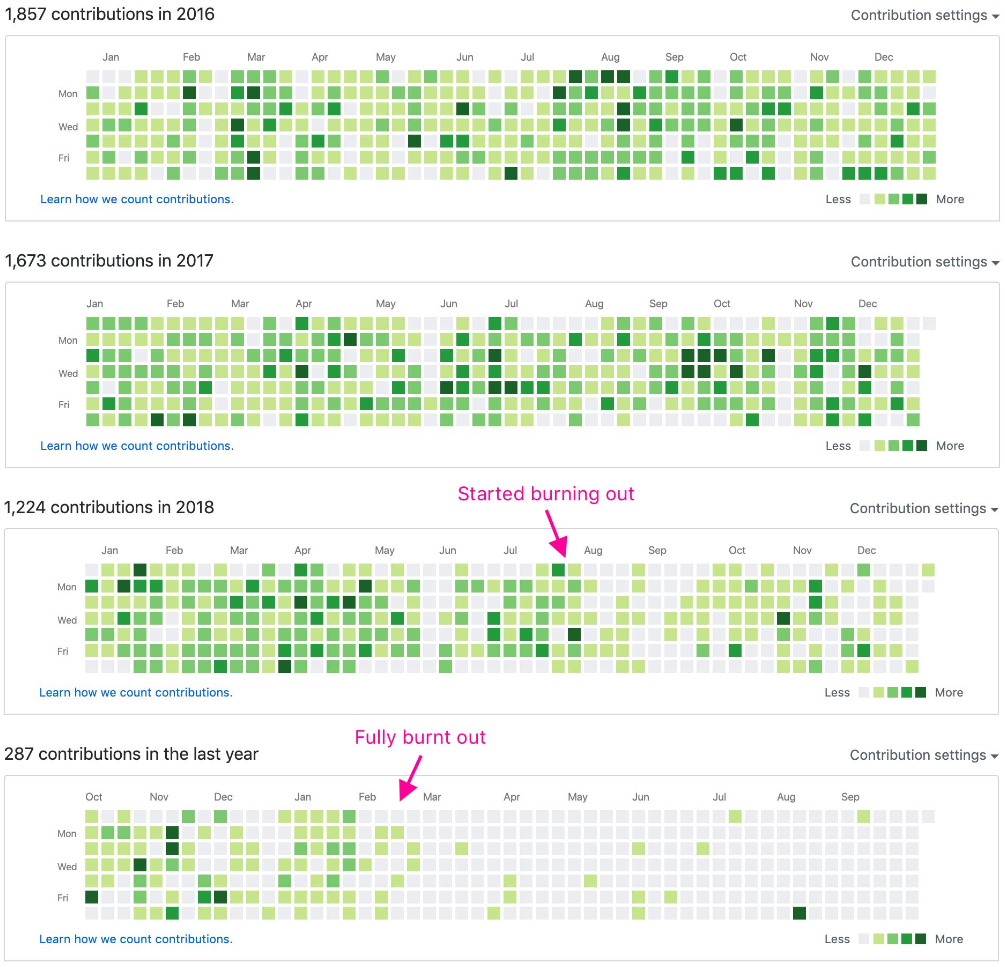
\includegraphics[width=0.7\textwidth]{burnout.png}
        \end{center}
    \end{frame}

    \begin{frame}
        \begin{center}
            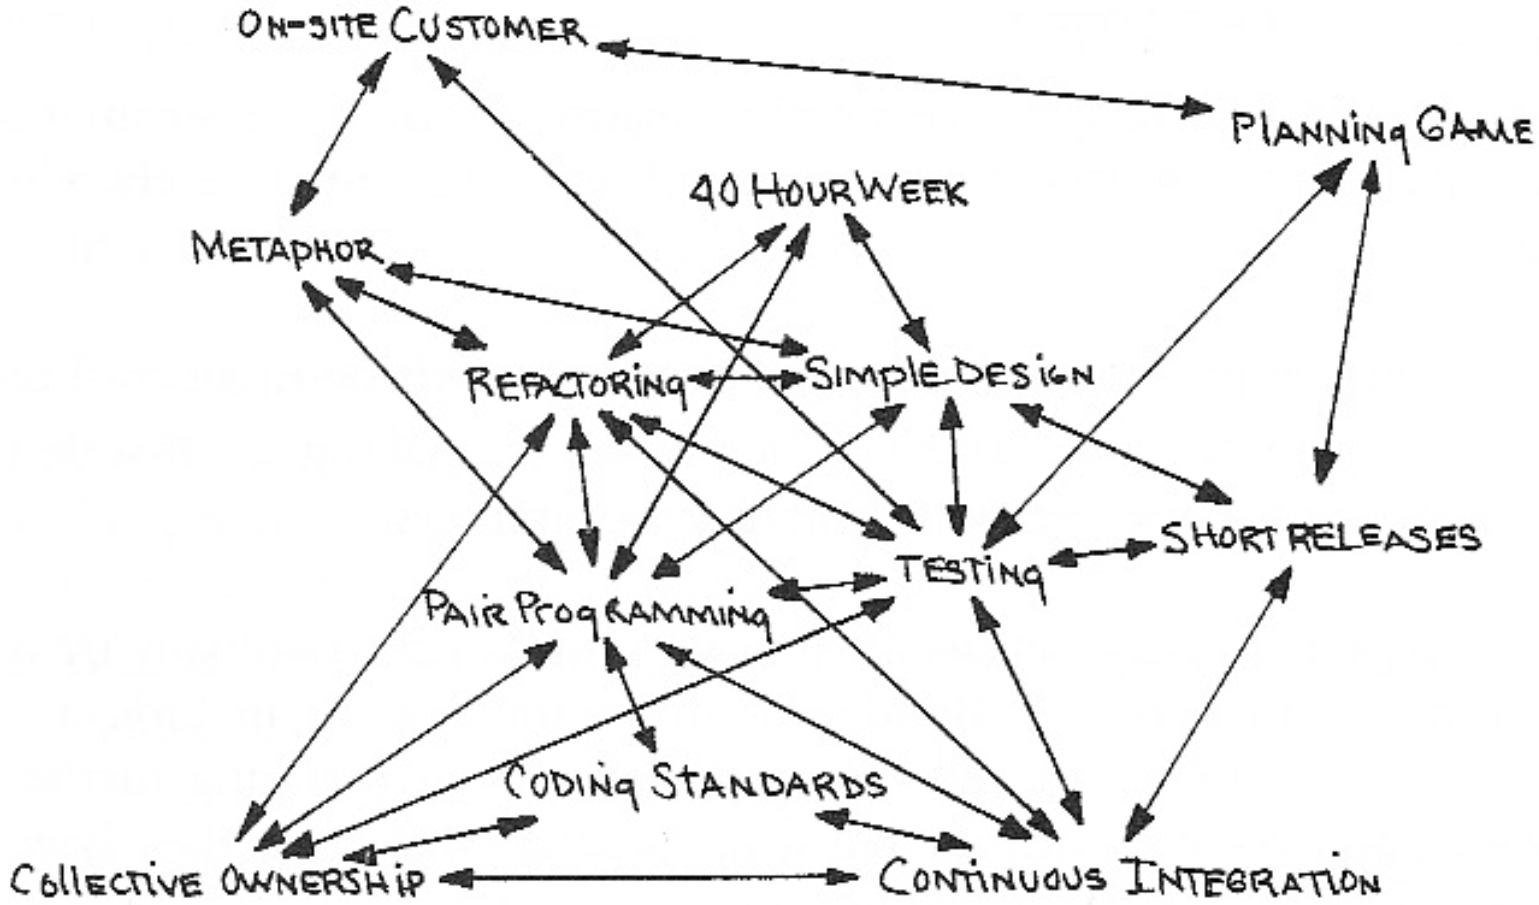
\includegraphics[width=0.9\textwidth]{xpPracticesRelationship.png}
        \end{center}
    \end{frame}

    \begin{frame}
        \frametitle{Процесс XP}
        \begin{center}
            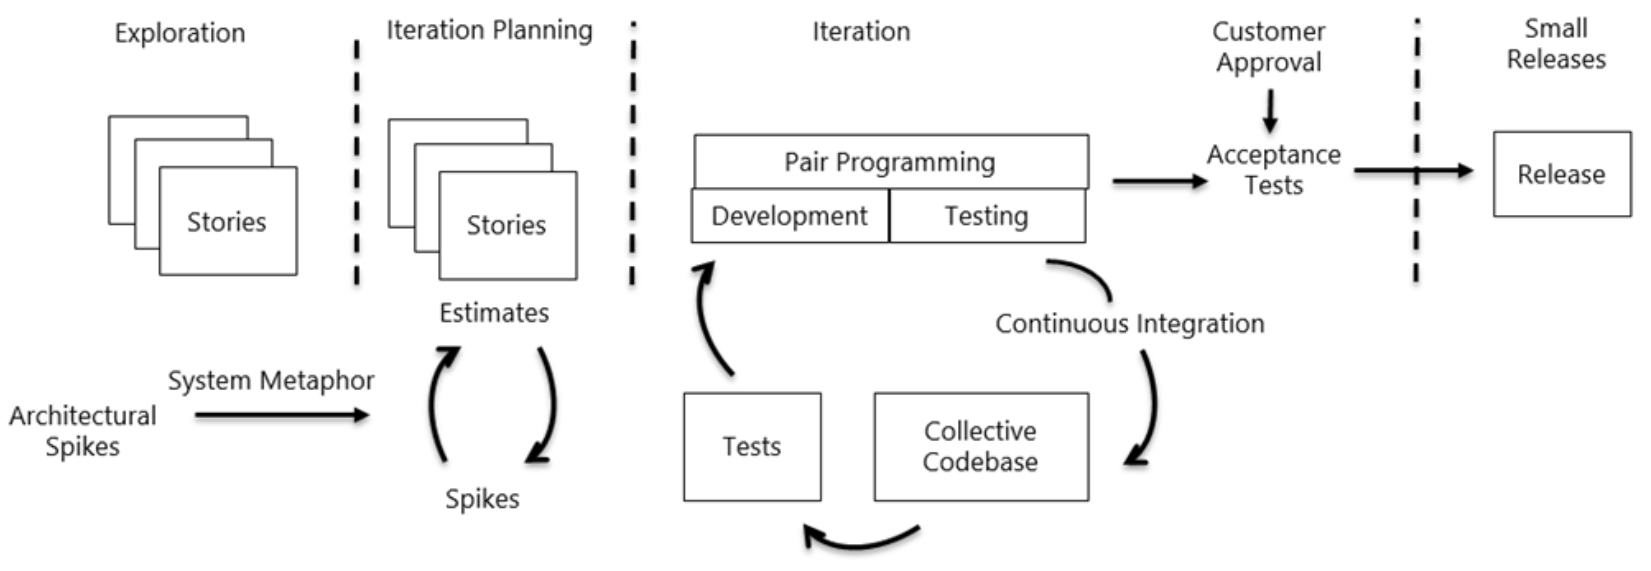
\includegraphics[width=0.9\textwidth]{xpProcess.png}
        \end{center}
    \end{frame}

    \begin{frame}
        \frametitle{Итерации в XP}
        \begin{center}
            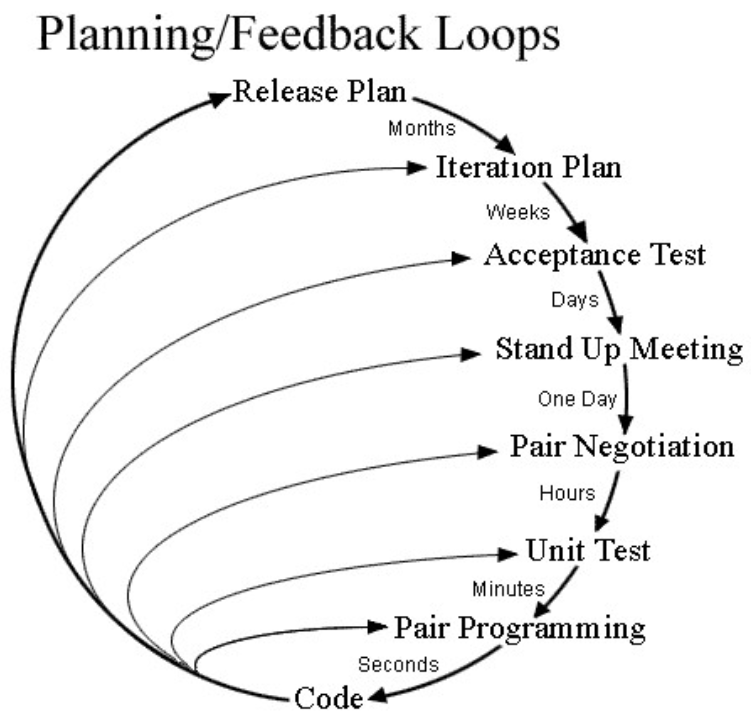
\includegraphics[width=0.5\textwidth]{xpIterations.png}
        \end{center}
    \end{frame}

    \begin{frame}
        \frametitle{XP: резюме}
        \begin{itemize}
            \item Применимость
            \begin{itemize}
                \item Небольшие и средние команды
                \item Неясные или быстро меняющиеся требования
            \end{itemize}
            \item Повышение доверия заказчика к программному продукту
            \item Минимизация ошибок на ранних стадиях
            \item Сокращение сроков разработки
            \item Повышение прогнозируемости
            \item Повышение качества ПО
        \end{itemize}
    \end{frame}

    \begin{frame}
        \frametitle{Критика XP}
        \begin{columns}
            \begin{column}{0.7\textwidth}
                \begin{itemize}
                    \item Высокие требования команде
                    \item Наличие заказчика в команде
                    \item Project scope creep
                    \item Постоянная переработка кода
                    \item Требования в виде приемочных тестов
                    \item Отсутствие целостного дизайна
                    \item Парное программирование
                \end{itemize}
            \end{column}
            \begin{column}{0.3\textwidth}
                \begin{center}
                    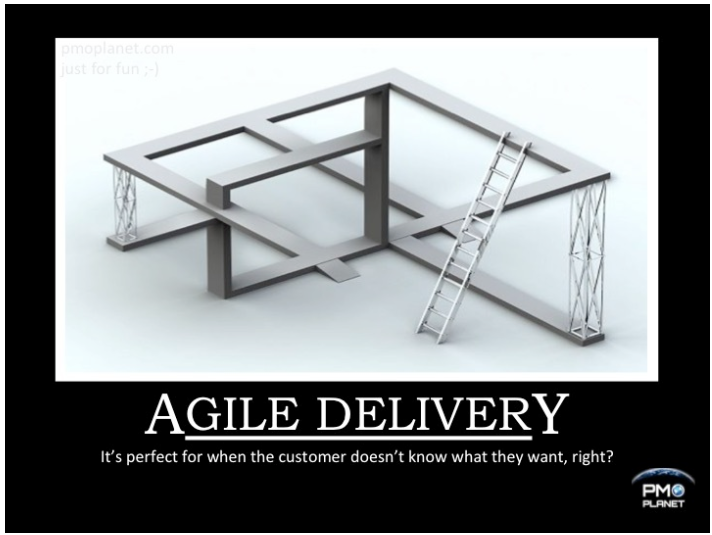
\includegraphics[width=\textwidth]{agileDelivery.png}
                \end{center}
            \end{column}
        \end{columns}
    \end{frame}

\end{document}
